\section{Domain Modeling}
\label{sec:Domain_Modeling}

\noindent This section describes the process of encoding of domain knowledge in OWL+SWRL, Prolog, and DTMC and PCTL templates. The application of these technologies is illustrated with respect to the UAV domain and, in particular, Mission~A, the example mission presented in the previous section.

\subsection{Semantic Modeling}
\label{sec:Semantic_Modeling}

\noindent With cascading verification, domain experts use ontologies to formally define domain concepts and their relationships. For our prototype, we have developed a \emph{complex missions ontology} (CEMO) that formalizes a subset of the UAV domain. Figure~\ref{fig:complex_missions_ontology} illustrates CEMO's class hierarchy, where each OWL class represents a grouping of individuals with similar characteristics. Five classes---\texttt{Action}, \texttt{Area}, \texttt{Asset}, \texttt{Mission} and \texttt{Waypoint}---inherit directly from the built-in OWL class \texttt{Thing}, which represents the set of all individuals. (The built-in OWL class \texttt{Nothing} represents the empty set.)

\begin{figure}
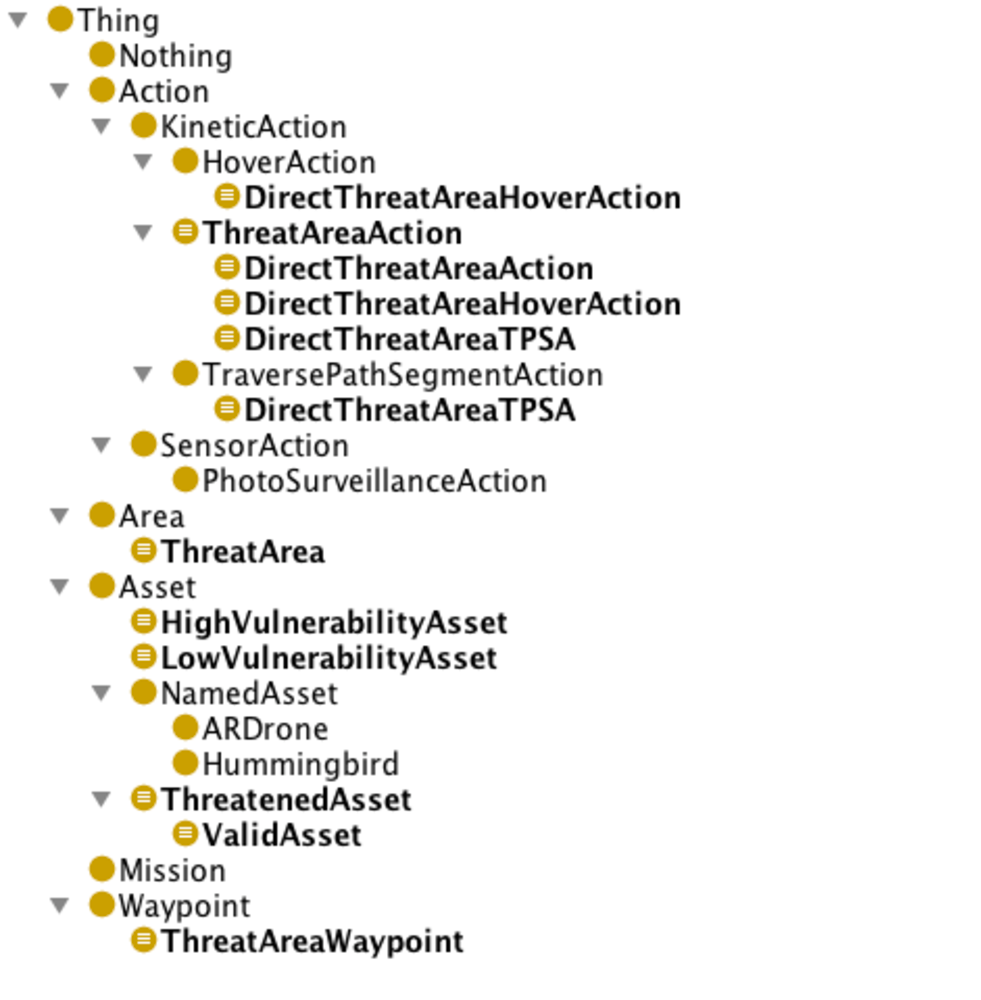
\includegraphics[scale=0.5]{img/cemo.pdf}
\caption{CEMO's class hierarchy as presented by the Prot\'eg\'e ontology editor.}
\label{fig:complex_missions_ontology}
\end{figure}

Having defined the concept of an asset we specify that every \texttt{Asset} individual must be associated with an \texttt{Action} individual via the \emph{object property} \texttt{hasAction}; in other words, every asset must execute at least one action. \texttt{Asset} individuals are also associated with \emph{data properties} that describe asset cost, endurance and speed. Class \texttt{Asset} is extended by classes \texttt{ARDrone} and \texttt{Hummingbird}. The latter classes represent quadcopter UAVs that have informed our research. Classes \texttt{Action}, \texttt{Asset} and \texttt{Hummingbird} are comprised in Mission~A (lines~1, 23 and~24, respectively, in Listing~\ref{lst:Mission_A}).

During a mission, assets execute actions that may be associated with other actions via \emph{preconditions}. An action~\emph{a} is a precondition to an action~\emph{b} if the end of~\emph{a} must precede the beginning of~\emph{b} in the sequence of actions that constitute an action workflow. Mission~A comprises three preconditions (lines~10, 18 and~22 in Listing~\ref{lst:Mission_A}), where each precondition relates actions assigned to the same asset. A fourth precondition (line~10) associates action \texttt{TPSA2} with action \texttt{TPSA3}, thereby coupling the behavior of the assets to which those actions are assigned (\texttt{H1} and~\texttt{H2}, respectively).

Class \texttt{Action} is extended by classes \texttt{KineticAction}, whose members are associated with a data property describing action duration, and \texttt{SensorAction}. Class \texttt{KineticAction} is in turn extended by classes \texttt{HoverAction} and \texttt{TraversePathSegmentAction}. The OWL code in Listing~\ref{lst:OWL_class_KineticAction} uses \emph{Manchester OWL syntax}---a human-friendly ontology representation language~\cite{Horridge_2006}---to formally define class \texttt{KineticAction}.

\begin{lstlisting}[caption={OWL code for class KineticAction},label=lst:OWL_class_KineticAction]
Class: KineticAction
  SubClassOf: Action
    and hasDurationInSeconds some int
    and hasPrecondition only Action
    (*\ldots*)
\end{lstlisting}

Listing~\ref{lst:OWL_class_KineticAction} contains the keywords \emph{some} (line~3) and \emph{only} (line~4), which represent, respectively, existential and universal restrictions in OWL\@. Existential restrictions describe classes of individuals that must participate in at least one relationship, along a specified property, with individuals that are members of a specified class~\cite{Horridge_2011}. Universal restrictions describe classes of individuals that may, and can only, participate in relationships along a specified property with individuals that are members of a specified class.

Assets may be required to commit threat area incursions, thereby compelling mission developers to consider the impact of asset \emph{survivability} on the probability of mission success. To accommodate this requirement, CEMO comprises classes that describe \emph{tactical} missions (Figure~\ref{fig:complex_missions_ontology} highlights these classes in bold). Used exclusively to support automated reasoning, tactical concepts are not available to mission developers via the YAML DSL\@. We note that the asset subtypes \texttt{HighVulnerabilityAsset} and \texttt{LowVulnerabilityAsset} are associated with a data property describing asset vulnerability. The specific value assigned to each subclass is used by the CVC to calculate probabilities that are ultimately integrated into DTMC models (the integration process will be elaborated in Section~\ref{sec:Behavioral_Modeling}).

\subsection{Rule-Based Modeling}
\label{sec:Rule_Based_Modeling}

\noindent OWL is a powerful knowledge representation formalism, but expressive and reasoning limitations constrain its utility; for example, OWL cannot model \emph{cross-cutting actions}. We consider an action~\emph{a} to be cross-cutting if~\emph{a} is a precondition to an action~\emph{b}, and~\emph{b} is assigned to an asset that is different from the asset to which~\emph{a} is assigned. By this definition, action \texttt{TPSA3} in Mission~A is a cross-cutting kinetic action. The OWL code in Listing~\ref{lst:OWL_class_CrossCuttingKineticAction} presents an incomplete definition of class \texttt{CrossCuttingKineticAction}.

\begin{lstlisting}[caption={OWL code for class CrossCuttingKineticAction},label=lst:OWL_class_CrossCuttingKineticAction]
Class: CrossCuttingKineticAction
  EquivalentTo: KineticAction
    and (isActionOf some Asset)
    and (hasPrecondition some
      (Action
        and (isActionOf some Asset)))
\end{lstlisting}

The definition in Listing~\ref{lst:OWL_class_CrossCuttingKineticAction} is lacking because the asset in line~3 cannot be differentiated from the asset in line~6. The SWRL code in Listing~\ref{lst:SWRL_rule_CrossCuttingKineticAction} uses the built-in OWL property \texttt{differentFrom} to appropriately define class \texttt{CrossCuttingKineticAction} (question mark prefixes denote variables).

\begin{lstlisting}[caption={SWRL code for rule CrossCuttingKineticAction},label=lst:SWRL_rule_CrossCuttingKineticAction]
Rule:
    KineticAction(?a), KineticAction(?b),
    Asset(?x), Asset(?y),
    hasAction(?x, ?a), hasAction(?y, ?b),
    hasPrecondition(?b, ?a),
    DifferentFrom(?x, ?y)
  -> CrossCuttingKineticAction(?a)
\end{lstlisting}

SWRL rules extend the expressive power of OWL; but like OWL, SWRL cannot reason effectively with negation. Rules that must reason with negation are therefore encoded in Prolog. Domain knowledge is negated during the ontology development process if Pellet reasoning with respect to that knowledge is deemed unattainable. The Prolog code in Listing~\ref{lst:Prolog_rule_terminal} formally defines rule \texttt{terminal}, which comprises three negated atoms (an atom is the basic building block of a Prolog rule). Rule \texttt{terminal} encapsulates both explicit and inferred ontological knowledge; explicit knowledge is encoded with the atom \texttt{has\_action} (line~2), while the three negated atoms (lines~3--5) encode knowledge inferred by Pellet.

\begin{lstlisting}[caption={Prolog code for rule terminal},label=lst:Prolog_rule_terminal]
terminal(X) :-
    has_action(A, X),
    not(is_precondition_to(X, _)),
    not(single_action_asset(A)),
    not(zero_action_asset(A)).
\end{lstlisting}

The transition of inferred knowledge from OWL to Prolog can be illustrated with the atom \texttt{is\_precondition\_to} (line~3 in Listing~\ref{lst:Prolog_rule_terminal}). The OWL code in Listing~\ref{lst:OWL_object_property_isPreconditionTo} formally defines the object property \texttt{isPreconditionTo}, a relationship that inverts the object property \texttt{hasPrecondition}. This inversion constitutes a Pellet inference.

\begin{lstlisting}[caption={OWL code for the object property isPreconditionTo},label=lst:OWL_object_property_isPreconditionTo]
ObjectProperty: isPreconditionTo
  InverseOf: hasPrecondition
  (*\ldots*)
\end{lstlisting}

Mission~A comprises several instances of the DSL construct \texttt{preconditions} (lines~10, 18 and~22 in Listing~\ref{lst:Mission_A}). The CVC transforms knowledge contained in this construct into knowledge encoded as property \texttt{hasPrecondition}. Knowledge inferred by Pellet with respect to \texttt{hasPrecondition}, via the inverted property \texttt{isPreconditionTo}, is transformed by the CVC into knowledge encoded with the atom \texttt{is\_precon\-dition\_to}, which in turn supports SWI-Prolog inferences.

\subsection{Behavioral Modeling}
\label{sec:Behavioral_Modeling}

\noindent OWL+SWRL and Prolog are appropriate formalisms for encoding semantic and rule-based knowledge. Likewise, the state-based PRISM modeling language is an appropriate formalism for encoding behavioral knowledge as DTMC models. The PRISM language can thus form the basis for re\-usable DTMC templates.

The code in Listing~\ref{lst:DTMC_asset_module_template} uses string interpolation---denoted by code snippet \texttt{\#\{ \ldots\ \}}---to encapsulate parameters in the context of a DTMC template for asset modules (the \emph{module} is a fundamental PRISM language construct). The asset module template encodes knowledge that describes the behavior of the \texttt{Asset} concept encoded in CEMO\@.

\begin{lstlisting}[caption={DTMC template for asset modules},label=lst:DTMC_asset_module_template]
module #{asset.class}#{asset.id}
  e#{asset.id} : [0..#{asset.endurance}]
      init #{asset.endurance};
  (*{\color{purple}{FOR action IN asset.kinetic\_actions}*)
  [#{action.type}]
      e#{asset.id}>0 &
      d#{action.id}>0
      -> (e#{asset.id}'=e#{asset.id}-1);
  (*{\color{purple}{END}*)
  [#{asset.last_action.type}]
      e#{asset.id}=0 |
      d#{asset.last_action.id}=0
      -> true;
endmodule
\end{lstlisting}

Arguments for the parameters in Listing~\ref{lst:DTMC_asset_module_template} are derived from explicit and inferred domain knowledge. Specifically, arguments for \texttt{asset.class} (line~1) and \texttt{asset.id} (lines~1, 2, 5, 7, and~9) are derived from mission plans; arguments for \texttt{asset.endurance} (lines~2 and~3) are derived from explicit domain knowledge encoded in CEMO; and arguments for \texttt{action.type} (line~5), \texttt{asset.last\_action.type} (line~9) and \texttt{asset.last\_action.id} (line~10) are derived from knowledge inferred by Pellet and the Prolog compiler (via a process that will be described in Section~\ref{sec:Cascading_Verification}).

A module definition contains \emph{variables} and \emph{commands}. Asset module states are stored in variable \texttt{e\#\{asset.id\}} (lines~2, 5, 7 and~9 in Listing~\ref{lst:DTMC_asset_module_template}), which represents asset endurance. Asset behavior is formalized with two or more commands, where each command assumes the form \texttt{[action] guard -> update}. A command becomes \emph{enabled} for execution when its \emph{guard} is satisfied by a specific model state. Commands encompass one or more updates, where each \emph{update} transitions a module, with a given probability, from one state to the next. A probability of one is assumed, and can therefore be omitted, for commands with single updates. Each command may be labeled with an \emph{action}, which forces two or more modules to transition states simultaneously (i.e., to synchronize).

Lines~4 and~8 in Listing~\ref{lst:DTMC_asset_module_template} use meta-code, which is highlighted with purple text, to define a for loop. Each asset module command generated by this loop represents the execution of a kinetic action. The \texttt{true} keyword in the last command (line~11) denotes the end of execution for a specific module. This type of command prevents deadlocks that are inconsequential to mission correctness from terminating the verification process with an error.

Asset module commands comprise single updates that o\-mit probabilities. The code in Listing~\ref{lst:DTMC_asset_survivability_template} formally defines a template for asset survivability modules, which contain commands with multiple updates (lines~12--15). The probability of execution for each update is derived from \texttt{asset.vulnerability}; arguments for this parameter are derived via inferences from explicit domain knowledge encoded in CEMO (as described in Section~\ref{sec:Semantic_Modeling}). Current vulnerability values are arbitrary, and should eventually be calculated from real-world data related to asset capabilities, terrain types and weather conditions.

\begin{lstlisting}[caption={DTMC template for asset survivability},label=lst:DTMC_asset_survivability_template]
(*{\color{purple}{FOR action IN asset.threat\_area\_actions}*)
formula actn#{action.id}_tai =
    d#{action.id}<=start#{action.id} &
    d#{action.id}>finish#{action.id};
(*{\color{purple}{END}*)

module #{asset.class}#{asset.id}_Survivability
  a#{asset.id}d : bool init false;
  (*{\color{purple}{FOR action IN asset.threat\_area\_actions}*)
  [#{action.type}] !a#{asset.id}d &
      actn#{action.id}_tai
      -> #{1-asset.vulnerability}
          :(a#{asset.id}d'=false) +
         #{asset.vulnerability}
          :(a#{asset.id}d'=true);
  [#{action.type}] a#{asset.id}d |
      !actn#{action.id}_tai
      -> true;
  (*{\color{purple}{END}*)
endmodule
\end{lstlisting}

Each survivability module enables PRISM to calculate the probability of survival for a threatened asset that has also been inferred by Pellet to be a \emph{valid asset}. The concept of a threatened asset was described in Section~\ref{sec:Method_Overview}; a valid asset is a threatened asset that executes at least one sensor action during a threat area incursion, thereby \emph{justifying} the risk assumed during that incursion.

The probability of survival for a valid asset is calculated with respect to \emph{threat area actions}, which are kinetic actions executed by the asset during threat area incursions. Lines~1 and~5 in Listing~\ref{lst:DTMC_asset_survivability_template} use meta-code to define a for loop that generates one PRISM formula with identifier \texttt{actn\#\{ac\-tion.id\}\_tai} per each action assigned to the asset in the loop header. Each formula specifies an overlap between the prosecution of a threat area incursion and the execution of a threat area action with identifier \texttt{action.id}. This overlap is delineated by variables \texttt{start\#\{action.id\}} and \texttt{finish\#\{action.id\}} (lines~3 and~4, respectively), which are assigned geographic information calculated by the CVC during preprocessing (as described in Section~\ref{sec:Method_Overview}).

The formula identifier \texttt{actn\#\{action.id\}\_tai} in Listing~\ref{lst:DTMC_asset_survivability_template} (defined in line~2 and used in lines~11 and~17) represents the execution of a kinetic action during the prosecution of a threat area incursion. The boolean variable \texttt{a\#\{asset.id\}d} (defined in line~8 and used in lines~10, 13, 15 and~16) represents the destruction of the asset with identifier \texttt{asset.id}. The constructs \texttt{actn\#\{action.id\}\_tai} and \texttt{a\#\{asset.id\}d} combine to form logical expressions, including a logical conjunction and disjunction (lines~10--11 and~16--17, respectively), that constitute the guards in the asset survivability module. When these expressions are considered in union, their logical truth values clarify asset behavior during threat area incursions. Specifically, a valid asset exists in one of the following disjoint states: 1) \emph{not} destroyed and prosecuting a threat area incursion (the logical conjunction); 2) destroyed, as a consequence of prosecuting a threat area incursion, or \emph{not} prosecuting a threat area incursion (the logical disjunction).

Mission properties are encoded in PRISM's property specification language, which subsumes several probabilistic temporal logics including PCTL, CSL and LTL\@. The code snippet \texttt{P=? [ F d\#\{action.id\}=0 \ldots\ ]} formally defines a mission property template. This generic property queries the probability that an action with identifier \texttt{action.id} will deplete its duration---as denoted by the assertion \texttt{d\#\{ac\-tion.id\}=0}---and thereby complete its execution. An ellipsis indicates the potential for synthesized properties to comprise multiple assertions. Output from PRISM templates will be presented in the following section.
